\documentclass{article}\usepackage[]{graphicx}\usepackage[]{color}
%% maxwidth is the original width if it is less than linewidth
%% otherwise use linewidth (to make sure the graphics do not exceed the margin)
\makeatletter
\def\maxwidth{ %
  \ifdim\Gin@nat@width>\linewidth
    \linewidth
  \else
    \Gin@nat@width
  \fi
}
\makeatother

\definecolor{fgcolor}{rgb}{0.345, 0.345, 0.345}
\newcommand{\hlnum}[1]{\textcolor[rgb]{0.686,0.059,0.569}{#1}}%
\newcommand{\hlstr}[1]{\textcolor[rgb]{0.192,0.494,0.8}{#1}}%
\newcommand{\hlcom}[1]{\textcolor[rgb]{0.678,0.584,0.686}{\textit{#1}}}%
\newcommand{\hlopt}[1]{\textcolor[rgb]{0,0,0}{#1}}%
\newcommand{\hlstd}[1]{\textcolor[rgb]{0.345,0.345,0.345}{#1}}%
\newcommand{\hlkwa}[1]{\textcolor[rgb]{0.161,0.373,0.58}{\textbf{#1}}}%
\newcommand{\hlkwb}[1]{\textcolor[rgb]{0.69,0.353,0.396}{#1}}%
\newcommand{\hlkwc}[1]{\textcolor[rgb]{0.333,0.667,0.333}{#1}}%
\newcommand{\hlkwd}[1]{\textcolor[rgb]{0.737,0.353,0.396}{\textbf{#1}}}%

\usepackage{framed}
\makeatletter
\newenvironment{kframe}{%
 \def\at@end@of@kframe{}%
 \ifinner\ifhmode%
  \def\at@end@of@kframe{\end{minipage}}%
  \begin{minipage}{\columnwidth}%
 \fi\fi%
 \def\FrameCommand##1{\hskip\@totalleftmargin \hskip-\fboxsep
 \colorbox{shadecolor}{##1}\hskip-\fboxsep
     % There is no \\@totalrightmargin, so:
     \hskip-\linewidth \hskip-\@totalleftmargin \hskip\columnwidth}%
 \MakeFramed {\advance\hsize-\width
   \@totalleftmargin\z@ \linewidth\hsize
   \@setminipage}}%
 {\par\unskip\endMakeFramed%
 \at@end@of@kframe}
\makeatother

\definecolor{shadecolor}{rgb}{.97, .97, .97}
\definecolor{messagecolor}{rgb}{0, 0, 0}
\definecolor{warningcolor}{rgb}{1, 0, 1}
\definecolor{errorcolor}{rgb}{1, 0, 0}
\newenvironment{knitrout}{}{} % an empty environment to be redefined in TeX

\usepackage{alltt}

\usepackage{comment}
\usepackage[english]{isodate}

\usepackage{graphicx}
\usepackage{siunitx}
\usepackage{paracol}
\usepackage{amsmath}
\usepackage{ amssymb }
\usepackage[utf8]{inputenc}
\usepackage[bookmarks=true]{hyperref}
\usepackage{bookmark}

\usepackage{mathtools,xparse}

\DeclarePairedDelimiter{\abs}{\lvert}{\rvert}
\DeclarePairedDelimiter{\norm}{\lVert}{\rVert}

\newcommand{\E}{\mathrm{E}}
\newcommand{\Var}{\mathrm{Var}}
\newcommand{\Cov}{\mathrm{Cov}}



\sisetup{output-decimal-marker = {,}}
\newcommand*{\ft}[1]{_\mathrm{#1}} 
\newcommand*{\dd}{\mathop{}\!\mathrm{d}}
\newcommand*{\tran}{^{\mkern-1.5mu\mathsf{T}}}%transpose of matrix
\newcommand{\trace}{\mathrm{trace}}
\IfFileExists{upquote.sty}{\usepackage{upquote}}{}
\begin{document}

	\begin{titlepage}
		\begin{center}
			\vspace*{1cm}
			\textbf{Math 423}\\
			\text{Linear Regression}\\
			\vspace{0.5cm}
			Homework II
			
			\vspace{1.5cm}
			
			\textbf{Frédéric Boileau}\\
			\vspace{2cm}
			Prof. 
			David A. Stephens
			\vfill
			\today
			\thispagestyle{empty}
		\end{center}
	\end{titlepage}
	
\section*{a}



\begin{knitrout}
\definecolor{shadecolor}{rgb}{0.969, 0.969, 0.969}\color{fgcolor}\begin{kframe}
\begin{alltt}
\hlkwd{require}\hlstd{(printr)}
\end{alltt}


{\ttfamily\noindent\itshape\color{messagecolor}{\#\# Loading required package: printr}}\begin{alltt}
\hlkwd{setwd}\hlstd{(}\hlkwd{dirname}\hlstd{(rstudioapi}\hlopt{::}\hlkwd{getActiveDocumentContext}\hlstd{()}\hlopt{$}\hlstd{path))}
\end{alltt}


{\ttfamily\noindent\bfseries\color{errorcolor}{\#\# Error: RStudio not running}}\begin{alltt}
\hlstd{salary}\hlkwb{<-}\hlkwd{read.csv}\hlstd{(}\hlstr{"salary.csv"}\hlstd{,}\hlkwc{header}\hlstd{=}\hlnum{TRUE}\hlstd{)}
\hlstd{x1}\hlkwb{<-}\hlstd{salary}\hlopt{$}\hlstd{SPENDING}\hlopt{/}\hlnum{1000}
\hlstd{y}\hlkwb{<-}\hlstd{salary}\hlopt{$}\hlstd{SALARY}
\end{alltt}
\end{kframe}
\end{knitrout}
we want to estimate the parameter $\beta_1$ and $\beta_0$, namely the slope and the intercept. We use the least square estimators. This is a case of simple linear regression so we can use the following equations:
\begin{equation} \hat\beta_1 = \frac{S_{xx}}{S_{xy}} \end{equation}

\begin{align} S_{xx}  &= \sum_{i=1}^{n}(x_i - \bar x)^2\\[2ex]
S_{xy} &= \sum_{i=1}^{n}y_i(x_i-\hat x) 
\end{align}\\[1ex]

\begin{equation} \hat\beta_0 = \bar y - \hat\beta_1 \hat x \end{equation}

\begin{knitrout}
\definecolor{shadecolor}{rgb}{0.969, 0.969, 0.969}\color{fgcolor}\begin{kframe}
\begin{alltt}
\hlstd{xbar} \hlkwb{=} \hlkwd{mean}\hlstd{(x1)}
\hlstd{ybar} \hlkwb{=} \hlkwd{mean}\hlstd{(y)}
\hlstd{Sxx} \hlkwb{=} \hlkwd{sum}\hlstd{((x1} \hlopt{-} \hlstd{xbar)}\hlopt{^}\hlnum{2}\hlstd{)}
\hlstd{Sxy} \hlkwb{=} \hlkwd{sum}\hlstd{(y}\hlopt{*}\hlstd{(x1} \hlopt{-} \hlstd{xbar))}
\hlstd{slope} \hlkwb{=} \hlstd{Sxy}\hlopt{/}\hlstd{Sxx}
\hlstd{intercept} \hlkwb{=} \hlstd{ybar} \hlopt{-} \hlstd{slope}\hlopt{*}\hlstd{xbar}
\hlkwd{print}\hlstd{(slope)}
\end{alltt}
\begin{verbatim}
## [1] 3307.585
\end{verbatim}
\begin{alltt}
\hlkwd{print}\hlstd{(intercept)}
\end{alltt}
\begin{verbatim}
## [1] 12129.37
\end{verbatim}
\begin{alltt}
\hlstd{fit.RP1} \hlkwb{=} \hlkwd{lm}\hlstd{(y}\hlopt{~}\hlstd{x1)}
\hlkwd{print}\hlstd{(}\hlkwd{coef}\hlstd{(fit.RP1))}
\end{alltt}
\begin{verbatim}
## (Intercept)          x1 
##   12129.371    3307.585
\end{verbatim}
\end{kframe}
\end{knitrout}

\clearpage

\section*{b and c}

The residual standard error is given by 
\begin{equation} \hat \sigma ^2 = \frac{SS_{\mathrm{Res}}}{n-2} \end{equation}
Moreover$SS_{\mathrm{Res}}$ is the sum of squares of error:

\begin{align}
SS_{\mathrm{Res}} = \sum_{i=1}^{n}(y_i - \hat y_i)^2 = \sum_{i=1}^{n}y_i^2 - n\hat y ^2 - \hat\beta_1 S_{xy}\\
= \sum_{i=1}^{n} (y_i - \bar y)^2  - \hat\beta_1 S_{xy}
\end{align}

\begin{knitrout}
\definecolor{shadecolor}{rgb}{0.969, 0.969, 0.969}\color{fgcolor}\begin{kframe}
\begin{alltt}
\hlstd{SSRes} \hlkwb{=} \hlkwd{sum}\hlstd{((y} \hlopt{-} \hlstd{ybar)}\hlopt{^}\hlnum{2}\hlstd{)} \hlopt{-} \hlstd{slope}\hlopt{*}\hlstd{Sxy}
\hlstd{n} \hlkwb{=} \hlkwd{length}\hlstd{(x1)}
\hlstd{residualStdError} \hlkwb{=} \hlkwd{sqrt}\hlstd{(SSRes}\hlopt{/}\hlstd{(n}\hlopt{-}\hlnum{2}\hlstd{))}
\hlkwd{print}\hlstd{(residualStdError)}
\end{alltt}
\begin{verbatim}
## [1] 2324.779
\end{verbatim}
\end{kframe}
\end{knitrout}

\section*{d}

We wish to compute the standard error with the values in the table already given. This table gives us the degrees of freedom (49) and the t value. 
\begin{equation} t_0 = \frac{\hat\beta_0}{\mathrm{se}(\hat\beta_0)} \Rightarrow 
\mathrm{se}(\hat\beta_0) = \frac{\hat\beta_0}{t_0} = \frac{12129.4}{10.13}  \end{equation}

Now to do the computation directly from the data we use the actual formula for the standard error which is given by
\begin{equation} \mathrm{se}(\hat\beta_1) = \sqrt{\frac{MS_{\mathrm{Res}}}{S_{xx}}} \qquad MS_{\mathrm{Res}} = \frac{SS_\mathrm{Res}}{n-2} = \hat\sigma^2 \end{equation}

\begin{knitrout}
\definecolor{shadecolor}{rgb}{0.969, 0.969, 0.969}\color{fgcolor}\begin{kframe}
\begin{alltt}
\hlstd{MSRes} \hlkwb{=} \hlstd{residualStdError} \hlopt{/} \hlkwd{sqrt}\hlstd{(n}\hlopt{-}\hlnum{2}\hlstd{)}
\hlkwd{print}\hlstd{(MSRes)}
\end{alltt}
\begin{verbatim}
## [1] 332.1113
\end{verbatim}
\end{kframe}
\end{knitrout}

\clearpage

\section*{e}


We will derive simple expressions from known relationships
	\begin{align*}
		SS_{\mathrm{Res}} &= SS_{\mathrm{T}} - \hat{\beta}_1 S_{xy}\\
		SS_{\mathrm{T}} &= SS_{\mathrm{R}} + SS_{\mathrm{Res}}\\ 
	\end{align*}
It is easy to see then that 
	\begin{align*}
		SS_{\mathrm{T}} &= SS_{\mathrm{Res}} + \hat \beta _1 S_{xy}\\
		SS_{\mathrm{R}} &=   \hat \beta _1 S_{xy}
	\end{align*}
	
	
\begin{knitrout}
\definecolor{shadecolor}{rgb}{0.969, 0.969, 0.969}\color{fgcolor}\begin{kframe}
\begin{alltt}
\hlstd{SST} \hlkwb{=} \hlstd{SSRes} \hlopt{+} \hlstd{slope}\hlopt{*}\hlstd{Sxy}
\hlstd{SSR} \hlkwb{=} \hlstd{slope}\hlopt{*}\hlstd{Sxy}
\hlstd{Rsqrd} \hlkwb{=} \hlstd{SSR}\hlopt{/}\hlstd{SST}
\hlkwd{print}\hlstd{(Rsqrd)}
\end{alltt}
\begin{verbatim}
## [1] 0.6967813
\end{verbatim}
\end{kframe}
\end{knitrout}


\section*{f}

\begin{knitrout}
\definecolor{shadecolor}{rgb}{0.969, 0.969, 0.969}\color{fgcolor}\begin{kframe}
\begin{alltt}
\hlstd{p} \hlkwb{=} \hlnum{2}
\hlstd{Fstat} \hlkwb{=} \hlstd{(SSR}\hlopt{/}\hlstd{(p}\hlopt{-}\hlnum{1}\hlstd{))}\hlopt{/}\hlstd{(SSRes}\hlopt{/}\hlstd{(n}\hlopt{-}\hlstd{p))}
\hlkwd{print}\hlstd{(Fstat)}
\end{alltt}
\begin{verbatim}
## [1] 112.5995
\end{verbatim}
\end{kframe}
\end{knitrout}
\clearpage


\section*{g}
\begin{align*}
	y\tran (I_n H_1)y = y\tran(I_n - H)y + y\tran(H-H_1)y 	
	\end{align*}
	
	The first statement we want to show is
	\begin{align*}
		\mathrm{trace}(I_n -H_1) = n-1
	\end{align*}
	Well the matrix $I_n$ has $a_{ii} = 1 \, \forall \, i\in [1,n]$ and $h _{ii} = 1/n \, \forall \, i \in [1,n]$
	By definitions:
	\begin{align}
		\mathrm{trace}(I_n-H_1) &= \sum_{i=1}^{n}(a_{ii} - h_{ii})\\[2ex]
		&= \sum_{i=1}^{n}(1-1/n)\\[2ex]
		&= n(1-1/n) = n-1
	\end{align}\\
	
	The second statement we need to prove is that:
	\begin{equation}
		\mathrm{trace}(H-H_1) = p-1
	\end{equation}
	We use the properties of the trace operator:
	\begin{align}
		\mathrm{trace}(H-H_1) &= \trace(H) - \trace(H_1)\\[2ex]
		\trace(H)&= \trace(X(X\tran X)^{-1}X\tran)\\
		&= \trace(X\tran X (X\tran X)^-1) \\
		&= \trace(I_p) \qquad \text{since} \quad X\tran X \in \mathbb{R}^{p\times p}\\
		&= p
	\end{align}
	As shown before the trace of $H_1$ is 1 and this with the previous derivation proves (13). 
\clearpage
\underline{Numerical part}


\begin{knitrout}
\definecolor{shadecolor}{rgb}{0.969, 0.969, 0.969}\color{fgcolor}\begin{kframe}
\begin{alltt}
\hlkwd{require}\hlstd{(MASS)}
\end{alltt}


{\ttfamily\noindent\itshape\color{messagecolor}{\#\# Loading required package: MASS}}

{\ttfamily\noindent\color{warningcolor}{\#\# Warning: package 'MASS' was built under R version 3.3.1}}\begin{alltt}
\hlstd{bigx} \hlkwb{=} \hlkwd{cbind}\hlstd{(}\hlkwd{matrix}\hlstd{(}\hlnum{1}\hlstd{,}\hlkwd{length}\hlstd{(x1)),x1)}

\hlstd{n1} \hlkwb{=}\hlkwd{length}\hlstd{(x1)}
\hlstd{H1} \hlkwb{=} \hlkwd{matrix}\hlstd{(}\hlnum{1}\hlopt{/}\hlstd{n1,n1,n1)}
\hlkwd{sum}\hlstd{(}\hlkwd{diag}\hlstd{((}\hlkwd{diag}\hlstd{(n1)} \hlopt{-} \hlstd{H1)))}
\end{alltt}
\begin{verbatim}
## [1] 50
\end{verbatim}
\begin{alltt}
\hlstd{H} \hlkwb{=} \hlstd{bigx} \hlopt  \hlkwd{ginv}\hlstd{(}\hlkwd{t}\hlstd{(bigx)} \hlopt \hlstd{bigx)} \hlopt \hlkwd{t}\hlstd{(bigx)}
\hlkwd{sum}\hlstd{(}\hlkwd{diag}\hlstd{(H} \hlopt{-} \hlstd{H1))}
\end{alltt}
\begin{verbatim}
## [1] 1
\end{verbatim}
\end{kframe}
\end{knitrout}



\clearpage
\section*{h}

\begin{knitrout}
\definecolor{shadecolor}{rgb}{0.969, 0.969, 0.969}\color{fgcolor}\begin{kframe}
\begin{alltt}
\hlstd{yhat} \hlkwb{=} \hlstd{intercept} \hlopt{+} \hlstd{slope}\hlopt{*}\hlstd{x1}
\hlstd{e} \hlkwb{=} \hlstd{y} \hlopt{-} \hlstd{yhat}
\hlkwd{plot}\hlstd{(x1,e)}
\end{alltt}
\end{kframe}
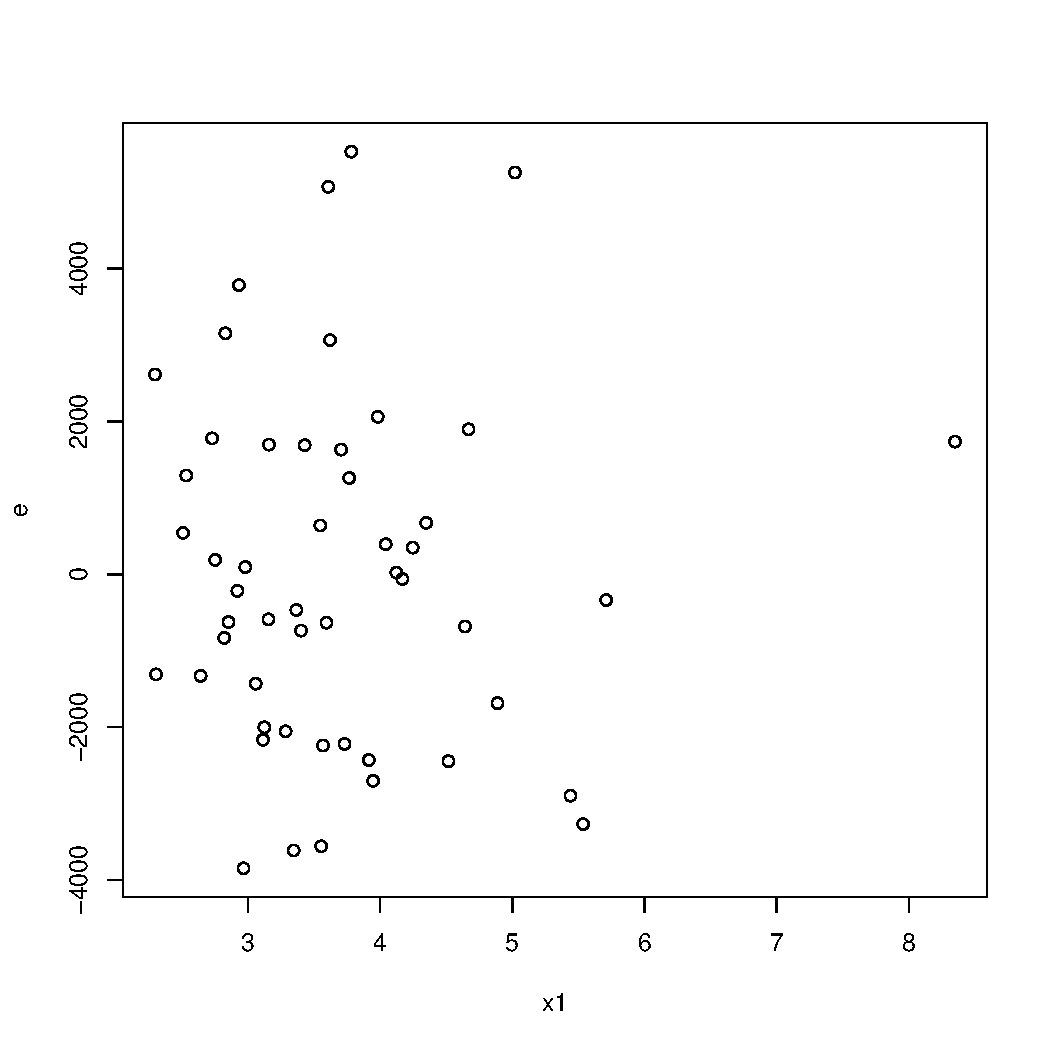
\includegraphics[width=\maxwidth]{figure/unnamed-chunk-8-1} 
\begin{kframe}\begin{alltt}
\hlkwd{mean}\hlstd{(x1)}
\end{alltt}
\begin{verbatim}
## [1] 3.696608
\end{verbatim}
\end{kframe}
\end{knitrout}
The residuals have zero mean.
\clearpage
\begin{knitrout}
\definecolor{shadecolor}{rgb}{0.969, 0.969, 0.969}\color{fgcolor}\begin{kframe}
\begin{alltt}
\hlkwd{boxplot}\hlstd{(x1[}\hlnum{1}\hlopt{:}\hlnum{10}\hlstd{],e[}\hlnum{1}\hlopt{:}\hlnum{10}\hlstd{],x1[}\hlnum{11}\hlopt{:}\hlnum{20}\hlstd{],e[}\hlnum{11}\hlopt{:}\hlnum{20}\hlstd{],x1[}\hlnum{21}\hlopt{:}\hlnum{30}\hlstd{],}
        \hlstd{e[}\hlnum{21}\hlopt{:}\hlnum{30}\hlstd{],x1[}\hlnum{31}\hlopt{:}\hlnum{40}\hlstd{],e[}\hlnum{31}\hlopt{:}\hlnum{40}\hlstd{],x1[}\hlnum{41}\hlopt{:}\hlnum{41}\hlstd{],e[}\hlnum{41}\hlopt{:}\hlnum{51}\hlstd{])}
\end{alltt}
\end{kframe}
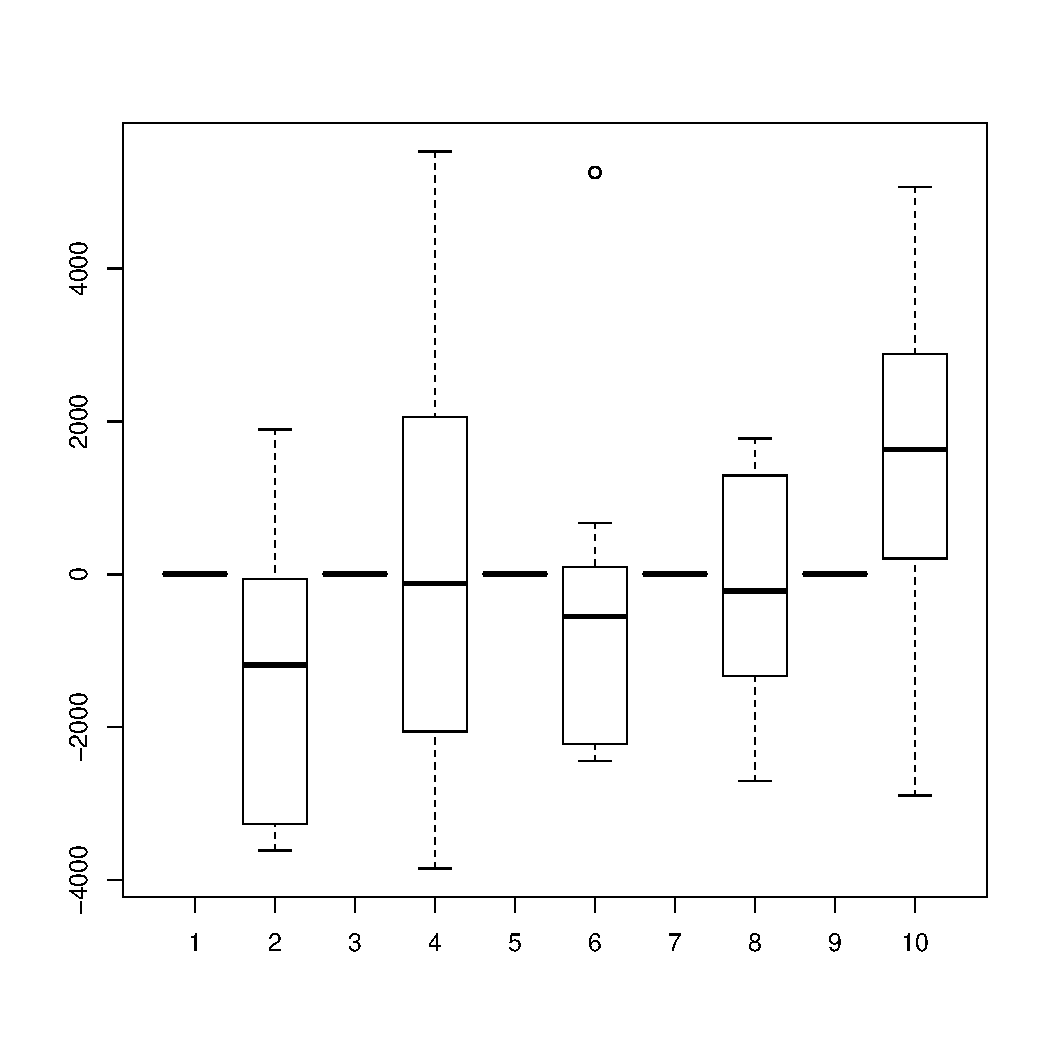
\includegraphics[width=\maxwidth]{figure/unnamed-chunk-9-1} 

\end{knitrout}
However a simple box plot shows quite clearly that they do not have constant variance. 
\clearpage
\begin{knitrout}
\definecolor{shadecolor}{rgb}{0.969, 0.969, 0.969}\color{fgcolor}\begin{kframe}
\begin{alltt}
\hlkwd{sum}\hlstd{(e)}\hlcom{#The sum of the residuals is zero, i.e. they are orthogonal to each other}
\end{alltt}
\begin{verbatim}
## [1] -8.731149e-11
\end{verbatim}
\begin{alltt}
\hlstd{bigx} \hlkwb{=} \hlkwd{cbind}\hlstd{(}\hlkwd{matrix}\hlstd{(}\hlnum{1}\hlstd{,}\hlkwd{length}\hlstd{(x1)),x1)}
\hlkwd{t}\hlstd{(bigx)}\hlopt\hlstd{e}\hlcom{#the residuals are orthogonal to the regressors}
\end{alltt}
\end{kframe}


\begin{tabular}{l|r}
\hline
 & 0\\
\hline
x1 & 0\\
\hline
\end{tabular}\begin{kframe}\begin{alltt}
\hlkwd{t}\hlstd{(yhat)}\hlopt\hlstd{e}\hlcom{#the residuals are orthogonal to the fitted values}
\end{alltt}
\end{kframe}


\begin{tabular}{r}
\hline
-2.4e-06\\
\hline
\end{tabular}
\end{knitrout}

\clearpage
\section*{i}
\begin{knitrout}
\definecolor{shadecolor}{rgb}{0.969, 0.969, 0.969}\color{fgcolor}\begin{kframe}
\begin{alltt}
\hlstd{prediction} \hlkwb{=} \hlstd{intercept} \hlopt{+} \hlstd{slope}\hlopt{*}\hlnum{4.8}
\hlkwd{print}\hlstd{(prediction)}
\end{alltt}
\begin{verbatim}
## [1] 28005.78
\end{verbatim}
\end{kframe}
\end{knitrout}

\section*{j}
	Let $x_0 :=x_1^{new} $
	\begin{align}
		\widehat{\E(y\vert x_0)} = \hat \mu_{u\vert x_0} = \hat \beta_0 +\hat \beta_1 x_0 \label{estimator_prediction}\\
	\end{align}
	The variance on a prediction is the variance of its estimator which is \ref{estimator_prediction}, so we compute as follows:
	\begin{align}
		\Var(\hat \mu_{y\vert x_0}) &= \Var(\hat \beta_0 + \hat \beta_1 x_0)\\[2ex]
		&= \Var [\bar y + \hat \beta_1 (x_0 - \bar x)]\\[2ex]
		&= \frac{\sigma^2}{n} + \frac{\sigma^2 (x_0-\bar x)^2}{S_{xx}}\\[2ex]
		&= \sigma^2 \left[\frac{1}{n} + \frac{(x_0-\bar x )^2}{S_{xx}}\right]
	\end{align}
	
	Now to estimate this value we use :
	\[\hat \sigma ^2 = MS_{Res}\]
	
	
	
\begin{knitrout}
\definecolor{shadecolor}{rgb}{0.969, 0.969, 0.969}\color{fgcolor}\begin{kframe}
\begin{alltt}
\hlstd{x1new} \hlkwb{=} \hlnum{4800}\hlopt{/}\hlnum{1000}
\hlstd{MSRes}\hlopt{*}\hlstd{(}\hlnum{1}\hlopt{/}\hlstd{n1}  \hlopt{+} \hlstd{(x1new} \hlopt{-} \hlstd{xbar)}\hlopt{^}\hlnum{2}\hlopt{/}\hlstd{Sxx)}
\end{alltt}
\begin{verbatim}
## [1] 13.78083
\end{verbatim}
\end{kframe}
\end{knitrout}











  
 


\end{document}
